\documentclass[a4paper, 12pt]{article} % Font size (can be 10pt, 11pt or 12pt) and paper size (remove a4paper for US letter paper)
\usepackage{amsmath,amsfonts,bm}
\usepackage{hyperref,verbatim}
\usepackage{amsthm,epigraph} 
\usepackage{amssymb}
\usepackage{framed,mdframed}
\usepackage{graphicx,color} 
\usepackage{mathrsfs,xcolor} 
\usepackage[all]{xy}
\usepackage{fancybox} 
% \usepackage{xeCJK}
\usepackage{CJKutf8}
\usepackage{pgf,tikz}
\usetikzlibrary{arrows}
\pagestyle{empty}
\definecolor{zzttqq}{rgb}{0.6,0.2,0}
\definecolor{uququq}{rgb}{0.25,0.25,0.25}
\definecolor{cqcqcq}{rgb}{0.75,0.75,0.75}
\newtheorem*{adtheorem}{定理}
% \setCJKmainfont[BoldFont=FZYaoTi,ItalicFont=FZYaoTi]{FZYaoTi}
\definecolor{shadecolor}{rgb}{1.0,0.9,0.9} %背景色为浅红色
\newenvironment{theorem}
{\bigskip\begin{mdframed}[backgroundcolor=gray!40,rightline=false,leftline=false,topline=false,bottomline=false]\begin{adtheorem}}
    {\end{adtheorem}\end{mdframed}\bigskip}
\newtheorem*{bdtheorem}{定义}
\newenvironment{definition}
{\bigskip\begin{mdframed}[backgroundcolor=gray!40,rightline=false,leftline=false,topline=false,bottomline=false]\begin{bdtheorem}}
    {\end{bdtheorem}\end{mdframed}\bigskip}
\newtheorem*{cdtheorem}{习题}
\newenvironment{exercise}
{\bigskip\begin{mdframed}[backgroundcolor=gray!40,rightline=false,leftline=false,topline=false,bottomline=false]\begin{cdtheorem}}
    {\end{cdtheorem}\end{mdframed}\bigskip}
\newtheorem*{ddtheorem}{注}
\newenvironment{remark}
{\bigskip\begin{mdframed}[backgroundcolor=gray!40,rightline=false,leftline=false,topline=false,bottomline=false]\begin{ddtheorem}}
    {\end{ddtheorem}\end{mdframed}\bigskip}
\newtheorem*{edtheorem}{引理}
\newenvironment{lemma}
{\bigskip\begin{mdframed}[backgroundcolor=gray!40,rightline=false,leftline=false,topline=false,bottomline=false]\begin{edtheorem}}
    {\end{edtheorem}\end{mdframed}\bigskip}
\newtheorem*{pdtheorem}{例}
\newenvironment{example}
{\bigskip\begin{mdframed}[backgroundcolor=gray!40,rightline=false,leftline=false,topline=false,bottomline=false]\begin{pdtheorem}}
    {\end{pdtheorem}\end{mdframed}\bigskip}

\usepackage[protrusion=true,expansion=true]{microtype} % Better typography
\usepackage{wrapfig} % Allows in-line images
\usepackage{mathpazo} % Use the Palatino font
\usepackage[T1]{fontenc} % Required for accented characters
\linespread{1.05} % Change line spacing here, Palatino benefits from a slight increase by default

\makeatletter
\renewcommand\@biblabel[1]{\textbf{#1.}} % Change the square brackets for each bibliography item from '[1]' to '1.'
\renewcommand{\@listI}{\itemsep=0pt} % Reduce the space between items in the itemize and enumerate environments and the bibliography

\renewcommand{\maketitle}{ % Customize the title - do not edit title
  % and author name here, see the TITLE block
  % below
  \renewcommand\refname{参考文献}
  \newcommand{\D}{\displaystyle}\newcommand{\ri}{\Rightarrow}
  \newcommand{\ds}{\displaystyle} \renewcommand{\ni}{\noindent}
  \newcommand{\pa}{\partial} \newcommand{\Om}{\Omega}
  \newcommand{\om}{\omega} \newcommand{\sik}{\sum_{i=1}^k}
  \newcommand{\vov}{\Vert\omega\Vert} \newcommand{\Umy}{U_{\mu_i,y^i}}
  \newcommand{\lamns}{\lambda_n^{^{\scriptstyle\sigma}}}
  \newcommand{\chiomn}{\chi_{_{\Omega_n}}}
  \newcommand{\ullim}{\underline{\lim}} \newcommand{\bsy}{\boldsymbol}
  \newcommand{\mvb}{\mathversion{bold}} \newcommand{\la}{\lambda}
  \newcommand{\La}{\Lambda} \newcommand{\va}{\varepsilon}
  \newcommand{\be}{\beta} \newcommand{\al}{\alpha}
  \newcommand{\dis}{\displaystyle} \newcommand{\R}{{\mathbb R}}
  \newcommand{\N}{{\mathbb N}} \newcommand{\cF}{{\mathcal F}}
  \newcommand{\gB}{{\mathfrak B}} \newcommand{\eps}{\epsilon}
  \begin{flushright} % Right align
    {\LARGE\@title} % Increase the font size of the title
    
    \vspace{50pt} % Some vertical space between the title and author name
    
    {\large\@author} % Author name
    \\\@date % Date
    
    \vspace{40pt} % Some vertical space between the author block and abstract
  \end{flushright}
}

% ----------------------------------------------------------------------------------------
%	TITLE
% ----------------------------------------------------------------------------------------
\begin{document}
\begin{CJK}{UTF8}{gkai}
  \title{\textbf{例12.7.2}}
  % \setlength\epigraphwidth{0.7\linewidth}
  \author{\small{叶卢庆}\\{\small{杭州师范大学理学院,学
        号:1002011005}}\\{\small{Email:h5411167@gmail.com}}} % Institution
  \renewcommand{\today}{\number\year. \number\month. \number\day}
  \date{\today} % Date
  
  % ----------------------------------------------------------------------------------------
  
  
  \maketitle % Print the title section
  
  % ----------------------------------------------------------------------------------------
  %	ABSTRACT AND KEYWORDS
  % ----------------------------------------------------------------------------------------
  
  % \renewcommand{\abstractname}{摘要} % Uncomment to change the name of the abstract to something else
  
  % \begin{abstract}
  
  % \end{abstract}
  
  % \hspace*{3,6mm}\textit{关键词:} % Keywords
  
  % \vspace{30pt} % Some vertical space between the abstract and first section
  
  % ----------------------------------------------------------------------------------------
  %	ESSAY BODY
  % ----------------------------------------------------------------------------------------
  \begin{example}[12.7.2]
    计算
$$
\int_0^1\int_0^{1-x}\sqrt{x+y}(y-2x)^2dydx.
$$    
\end{example}
\begin{proof}[解]
  如上积分的区域为
$$
0\leq x\leq 1,0\leq y\leq 1-x.
$$
画出的图像如下:\\
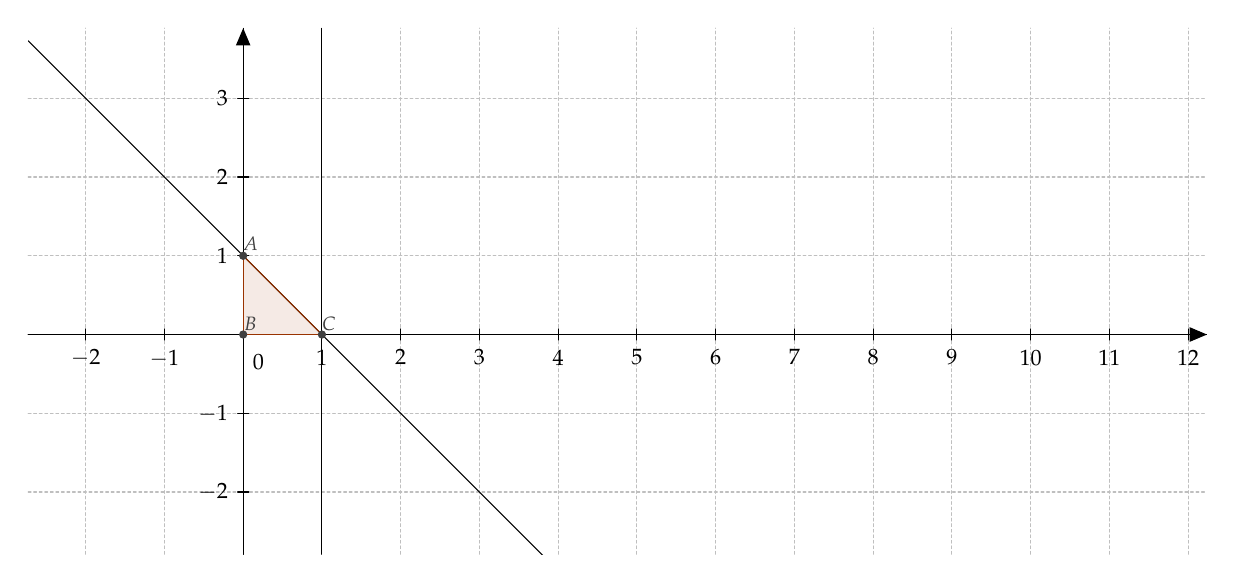
\begin{tikzpicture}[line cap=round,line join=round,>=triangle
  45,x=1.0cm,y=1.0cm]
  \draw [color=cqcqcq,dash pattern=on 1pt off 1pt,
  xstep=1.0cm,ystep=1.0cm] (-2.73,-2.79) grid (12.24,3.89);
  \draw[->,color=black] (-2.73,0) -- (12.24,0); \foreach \x in
  {-2,-1,1,2,3,4,5,6,7,8,9,10,11,12} \draw[shift={(\x,0)},color=black]
  (0pt,2pt) -- (0pt,-2pt) node[below] {\footnotesize $\x$};
  \draw[->,color=black] (0,-2.79) -- (0,3.89); \foreach \y in
  {-2,-1,1,2,3} \draw[shift={(0,\y)},color=black] (2pt,0pt) --
  (-2pt,0pt) node[left] {\footnotesize $\y$}; \draw[color=black]
  (0pt,-10pt) node[right] {\footnotesize $0$}; \clip(-2.73,-2.79)
  rectangle (12.24,3.89); \fill[color=zzttqq,fill=zzttqq,fill
  opacity=0.1] (0,1) -- (0,0) -- (1,0) -- cycle; \draw (0,-2.79) --
  (0,3.89); \draw (1,-2.79) -- (1,3.89); \draw [domain=-2.73:12.24]
  plot(\x,{(-0-0*\x)/1}); \draw [domain=-2.73:12.24]
  plot(\x,{(--1-1*\x)/1}); \draw [color=zzttqq] (0,1)-- (0,0); \draw
  [color=zzttqq] (0,0)-- (1,0); \draw [color=zzttqq] (1,0)-- (0,1);
  \begin{scriptsize}
    \fill [color=uququq] (0,1) circle (1.5pt); \draw[color=uququq]
    (0.09,1.15) node {$A$}; \fill [color=uququq] (0,0) circle (1.5pt);
    \draw[color=uququq] (0.09,0.14) node {$B$}; \fill [color=uququq]
    (1,0) circle (1.5pt); \draw[color=uququq] (1.09,0.14) node {$C$};
  \end{scriptsize}
\end{tikzpicture}
令 $u=\sqrt{x+y}$,$v=y-2x$.则
$$
\begin{cases}
  x+y=u^2,\\
  y-2x=v.\\
\end{cases}
$$
因此
$$
\begin{cases}
  x=\frac{u^2-v}{3},\\
y=\frac{2}{3}u^2+\frac{1}{3}v.
\end{cases}
$$
易得 Jacobi 矩阵为
$$
\begin{pmatrix}
  \frac{\pa x}{\pa u}&\frac{\pa x}{\pa v}\\
\frac{\pa y}{\pa u}&\frac{\pa y}{\pa v}
\end{pmatrix}=\begin{pmatrix}
  \frac{2}{3}u&\frac{-1}{3}\\
\frac{4}{3}u&\frac{1}{3}
\end{pmatrix}=\frac{2}{3}u.
$$
只有在 $u=0$ 时才为0,也就是只有在 $x+y=0$ 时才为0,而在 $xy$ 平面上,直
线 $y=-x$ 的测度为0.\\

且
$$
0\leq \frac{u^2-v}{3}\leq 1,0\leq \frac{2}{3}u^2+\frac{1}{3}v\leq 1-(\frac{u^2-v}{3}).
$$
也即
$$
0\leq u\leq 1,-2u^2\leq v\leq u^2.
$$

图像如下,是最深蓝色的部分的左边部分:\\
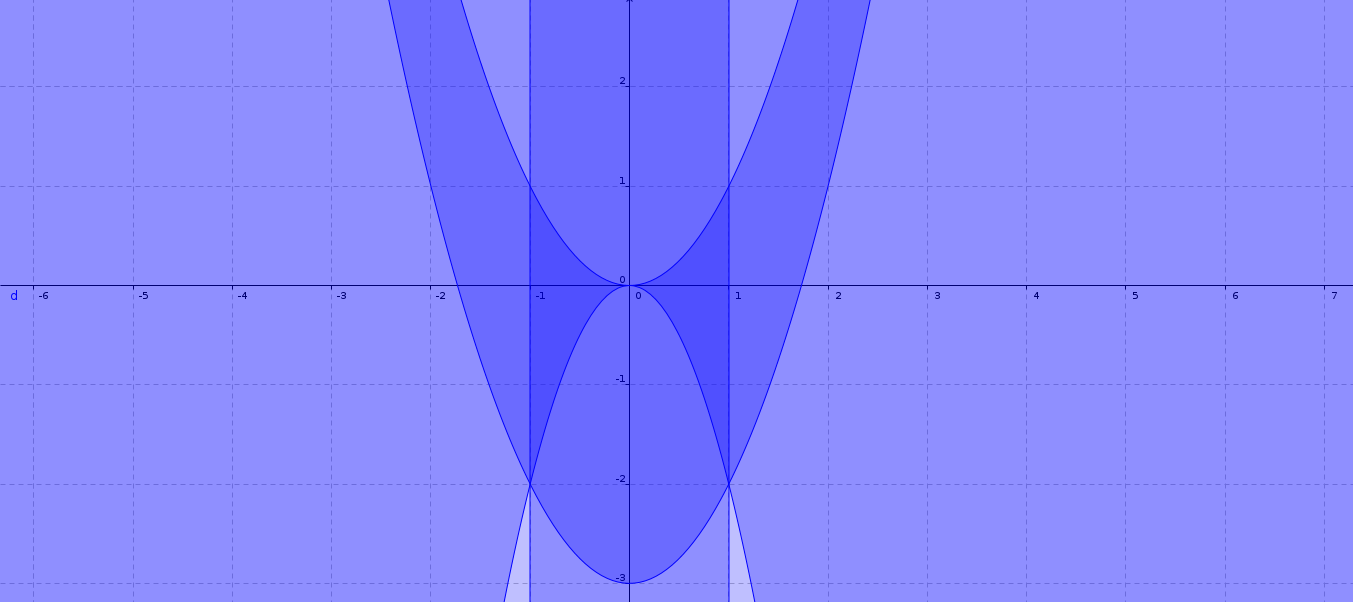
\includegraphics[width=1\textwidth]{/home/luqing/Thomas-calculus-10th-edition/example12-7-2.png}
易知
$$
\int_0^1\int_0^{1-x}\sqrt{x+y}(y-2x)^2dydx=\int_{0}^1\int_{-2u^2}^{u^2}\frac{2}{3}u^2v^2dvdu=\frac{2}{9}.
$$    
\end{proof}
% ----------------------------------------------------------------------------------------
% BIBLIOGRAPHY
% ----------------------------------------------------------------------------------------
  
\bibliographystyle{unsrt}
  
\bibliography{sample}
  
% ----------------------------------------------------------------------------------------
\end{CJK}
\end{document}